%% Dokumentenklasse (Koma Script)
\documentclass[%
   %draft,     % Entwurfsstadium
   final,      % fertiges Dokument
%%%% --- Schriftgröße ---
   11pt,
%%%% --- Sprache ---
   english,
   ngerman,           % Letzte Sprache ist die Hauptsprache, andere muss erst ausgewählt werden.
%%%% === Seitengröße ===
   a4paper,
%%%% === Optionen für den Satzspiegel ===
   %BCOR5mm,         % Zusaetzlicher Rand auf der Innenseite (Bindekorrektur)
   %DIV11,           % Seitengroesse (siehe Koma Skript Dokumentation!)
   %DIVcalc,         % automatische Berechnung einer guten Zeilenlaenge
   1.1headlines,     % Zeilenanzahl der Kopfzeilen
   %headinclude,     % Kopf einbeziehen
   headinclude=false,      % Kopf nicht einbeziehen
   %footinclude,     % Fuss einbeziehen
   footinclude=false,      % Fuss nicht einbeziehen
   %mpinclude,       % Margin einbeziehen
   mpinclude=false,        % Margin nicht einbeziehen
   pagesize,         % Schreibt die Papiergroesse in die Datei.
                     % Wichtig fuer Konvertierungen
%%%% === Layout ===
   %oneside,          % einseitiges Layout
   twoside,         % Seitenraender für zweiseitiges Layout
   onecolumn,        % Einspaltig
   %twocolumn,       % Zweispaltig
   %openany,         % Kapitel beginnen auf jeder Seite
   %openright,        % Kapitel beginnen immer auf der rechten Seite
                     % (macht nur bei 'twoside' Sinn)
   %cleardoubleplain,    % leere, linke Seite mit Seitenstil 'plain'
   %cleardoubleempty,    % leere, linke Seite mit Seitenstil 'empty'
   titlepage,        % Titel als einzelne Seite ('titlepage' Umgebung)
   %notitlepage,     % Titel in Seite integriert
%%%% --- Absatzeinzug ---
   %                 % Absatzabstand: Einzeilig,
   %parskip,         % Freiraum in letzter Zeile: 1em
   %parskip*,        % Freiraum in letzter Zeile: Viertel einer Zeile
   %parskip+,        % Freiraum in letzter Zeile: Drittel einer Zeile
   %parskip-,        % Freiraum in letzter Zeile: keine Vorkehrungen
   %                 % Absatzabstand: Halbzeilig
   %halfparskip,     % Freiraum in letzter Zeile: 1em
   %halfparskip*,    % Freiraum in letzter Zeile: Viertel einer Zeile
   %halfparskip+,    % Freiraum in letzter Zeile: Drittel einer Zeile
   parskip=half,      % Freiraum in letzter Zeile: keine Vorkehrungen
   %                 % Absatzabstand: keiner
   %parindent,       % Eingerückt (Standard)
%%%% --- Kolumnentitel ---
   headsepline,      % Linie unter Kolumnentitel
   %headnosepline,   % keine Linie unter Kolumnentitel
   %footsepline,     % Linie unter Fussnote
   %footnosepline,   % keine Linie unter Fussnote
%%%% --- Kapitel ---
   %chapterprefix,   % Ausgabe von 'Kapitel:'
   chapterprefix=false,
   version=first,  % keine Ausgabe von 'Kapitel:'
%%%% === Verzeichnisse (TOC, LOF, LOT, BIB) ===
   listof=totoc,      % Tabellen & Abbildungsverzeichnis ins TOC
   %idxtotoc,        % Index ins TOC
   bibliography=totoc,
   verson=first,         % Bibliographie ins TOC
   %bibtotocnumbered, % Bibliographie im TOC nummeriert
   %liststotocnumbered, % Alle Verzeichnisse im TOC nummeriert
   toc=graduated,        % eingereuckte Gliederung
   %tocleft,         % Tabellenartige TOC
   %listsindent,      % eingereuckte LOT, LOF
   %listsleft,       % Tabellenartige LOT, LOF
   %pointednumbers,  % Überschriftnummerierung mit Punkt, siehe DUDEN !
   %pointlessnumbers, % Überschriftnummerierung ohne Punkt, siehe DUDEN !
   %openbib,         % alternative Formatierung des Literaturverzeichnisses
%%%% === Matheformeln ===
   %leqno,           % Formelnummern links
   fleqn,            % Formeln werden linksbuendig angezeigt
]{scrbook}%     Klassen: scrartcl, scrreprt, scrbook
% -------------------------------------------------------------------------

% -------------- Daten f�r die Titelseite --> diese m�ssen angepasst werden!
\newcommand*{\thedockind}{Bachelor-/Masterthesis}
\newcommand*{\thetitle}{Hier der Titel der Arbeit}
\newcommand*{\thesubtitle}{Sofern vorhanden, hier der Untertitel. Dieser kann auch etwas l�nger sein...}
\newcommand*{\theauthor}{Student Name}
\newcommand*{\thematriculationnumber}{123456789} % Matrikelnummer
\newcommand*{\thebirthday}{15.09.1988} % Geburtstag
\newcommand*{\thedegree}{Bachelor/Master of Science}
\newcommand*{\themajor}{Praktische Informatik} % Studiengang
\newcommand*{\thedate}{\today} % \today kann durch ein Datum erstetzt werden.
\newcommand*{\thebetreuer}{Prof. Dr. Sabine Sachweh}
\newcommand*{\thezweitbetreuer}{Name Zweitpr�fer}
% -------------- Ende Daten f�r die Titelseite

%%% Doc: ftp://tug.ctan.org/pub/tex-archive/macros/latex/required/babel/babel.pdf
% Languagesetting
\usepackage{babel}	% Sprache

\usepackage{textpos} 


\usepackage{fixltx2e}	% Verbessert einige Kernkompetenzen von LaTeX2e
\usepackage{ellipsis}	% Korrigiert den Wei�raum um Auslassungspunkte

\usepackage{placeins} 

\usepackage{ifpdf}
\ifpdf
\pdfinfo {
	/Author (\theauthor)
	/Title (\thetitle)
	/Subject ()
	/Keywords ()
%	/CreationDate (D:YYYYMMTTHHMMSS)
}
\fi



%%% Doc: www.cs.brown.edu/system/software/latex/doc/calc.pdf
% Calculation with LaTeX
\usepackage{calc}

%%% Doc: ftp://tug.ctan.org/pub/tex-archive/macros/latex/contrib/xcolor/xcolor.pdf
% Farben
% Incompatible: Do not load when using pstricks !
\usepackage[
	table % Load for using rowcolors command in tables
]{xcolor}

\usepackage{tikz}
\usetikzlibrary{% 
   arrows,% 
   calc,% 
   fit,% 
   patterns,% 
   plotmarks,% 
   shapes.geometric,% 
   shapes.misc,% 
   shapes.symbols,% 
   shapes.arrows,% 
   shapes.callouts,% 
   shapes.multipart,% 
   shapes.gates.logic.US,% 
   shapes.gates.logic.IEC,% 
   er,% 
   automata,% 
   backgrounds,% 
   chains,% 
   topaths,% 
   trees,% 
   petri,% 
   mindmap,% 
   matrix,% 
   calendar,% 
   folding,% 
   fadings,% 
   through,% 
   positioning,% 
   scopes,% 
   decorations.fractals,% 
   decorations.shapes,% 
   decorations.text,% 
   decorations.pathmorphing,% 
   decorations.pathreplacing,% 
   decorations.footprints,% 
   decorations.markings,% 
   shadows} 
   
%%% Doc: ftp://tug.ctan.org/pub/tex-archive/macros/latex/required/graphics/grfguide.pdf
% Bilder
\usepackage[%
	%final,
	%draft % do not include images (faster)
]{graphicx}


% bessere Abstaende innerhalb der Tabelle (Layout))
% -------------------------------------------------
%%% Doc: ftp://tug.ctan.org/pub/tex-archive/macros/latex/contrib/booktabs/booktabs.pdf
\usepackage{booktabs}


%%% Doc: ftp://tug.ctan.org/pub/tex-archive/macros/latex/contrib/enumitem/enumitem.pdf
% Better than 'paralist' and 'enumerate' because it uses a keyvalue interface!
% Do not load together with enumerate.
%\usepackage{enumitem}

\usepackage{paralist}


%%% Doc: http://www.ctan.org/tex-archive/macros/latex/contrib/acronym/acronym.pdf
% Usage:
%        Definition: \acro{ acronym }[ short name ]{ full name }
%        Nutzung im Text: \ac{acronym}
 \usepackage[
 	%footnote,	% Full names appear in the footnote
 	%smaller,		% Print acronym in smaller fontsize
 	%printonlyused %
 ]{acronym}
%\chapter*{Abkürzungsverzeichnis}
\addcontentsline{toc}{chapter}{Abkürzungsverzeichnis}  
\begin{acronym}[Visual Studio] %Längster Begriff
\setlength{\itemsep}{-\parsep}
	\acro{.apk}{Android Package}
	\acro{ACL}{Access Control Lists}
	\acro{AES}{Advanced Encryption Standard}
	\acro{AJAX}{Asynchronous JavaScript and XML}	
	\acro{ANR}{Application Not Responding}
	\acro{API}{Application Programming Interface}
	\acro{CORS}{Cross-origin resource sharing}
	\acro{CRUD}{Create Read Update Delete}	
	\acro{CSS}{Cascading Style Sheet}
	\acro{DLL}{Dynamic Link Library}
	\acro{DRAM}{Dynamischer \ac{RAM}}
	\acro{HTML}{Hypertext Markup Language}	
	\acro{HTTP}{Hypertext Transfer Protocol}	
	\acro{HTTPS}{Hyper Text Transfer Protocol Secure}	
	\acro{IDE}{Integrated Development Environment}
	\acro{JSON}{JavaScript Object Notation}	
	\acro{JWT}{\ac{JSON} Web Token}	
	\acro{MSSQL}{Microsoft SQL Server}
	\acro{MVC}{Model-View-Controller}	
	\acro{MVVM}{Model-View-ViewModel}
	\acro{OR-Mapper}{objekt-relationaler Mapper}
	\acro{PCL}{Portable Class Library}
	\acro{RAM}{Random Access Memory}
	\acro{RBAC}{Role Based Access Control}	
	\acro{REST}{Representational State Transfer}	
	\acro{SPA}{Single Page Application}
	\acro{SRAM}{Statischer \ac{RAM}}
	\acro{TCP}{Transmission Control Protocol}
	\acro{URI}{Uniform Resource Identifier}		
	\acro{URL}{Uniform Resource Locator}		
	\acro{Visual Studio}{Microsoft Visual Studio 2015 Community Edition}		
	\acro{VM}{Virtuelle Maschine}
	\acro{Web-App}{mobil-optimierte Webseite}
	\acro{XML}{Extensible Markup Language}
\end{acronym}



%% Kopf und Fusszeilen====================================================
%%% Doc: ftp://tug.ctan.org/pub/tex-archive/macros/latex/contrib/koma-script/scrguide.pdf
\usepackage[%
   automark,         % automatische Aktualisierung der Kolumnentitel
   %nouppercase,      % Grossbuchstaben verhindern
   %markuppercase    % Grossbuchstaben erzwingen
   %markusedcase     % vordefinierten Stil beibehalten
   %komastyle,       % Stil von Koma Script
   %standardstyle,   % Stil der Standardklassen
]{scrpage2}



%% UeberSchriften (Chapter und Sections) =================================
% -- Ueberschriften komlett Umdefinieren --
%%% Doc: ftp://tug.ctan.org/pub/tex-archive/macros/latex/contrib/titlesec/titlesec.pdf
\usepackage{titlesec}

% -- Section Aussehen veraendern --
% --------------------------------
%% -> Section mit Unterstrich
% \titleformat{\section}
%   [hang]%[frame]display
%   {\usekomafont{sectioning}\Large}
%  {\thesection}
%   {6pt}
%   {}
%   [\titlerule \vspace{0.5\baselineskip}]
% --------------------------------

% -- Chapter Aussehen veraendern --
% --------------------------------
\titleformat{\chapter}[block]	% {command}[shape]
  {\usekomafont{chapter}\huge\sffamily\bfseries}	% format
  {   										% label
  {\thechapter.} \filright%
  }%}
  {1pt}										% sep (from chapternumber)
  {\vspace{0.5pc} \filright}   % {before}[after] (before chaptertitle and after)
  [\vspace{0.5pc} \filright {}]

% \titleformat{\chapter}[]%
%    {\usekomafont{chapter}\huge\sffamily\bfseries}%
%    {\thechapter}%
%    {1em}%
%    {}%


\usepackage{rotating}

%Literatur-Einstellungen

%vielleicht Layout anpassen...

\usepackage[%
style=authortitle-dw,
namefont=smallcaps,%
firstnamefont=smallcaps,%
idemfont=smallcaps,% Schriftart von »Ders.« / »Dies.«
%ibidemfont=smallcaps,% Schriftart von »ebenda« / »ebd.«
idembib=true,% aufeinanderfolgende Einträge -> »Ders.« bzw. »Dies.«
idembibformat=idem,% idem= Ders./Dies.; alternativ: =dash macht Strich -
edbyidem=true,% Autor und Herausgeber bei @incollection- oder @inbook- Einträgen dieselben
nopublisher=true,% true unterdrückt den Verlag
%nolocation=true,% true unterdrückt den Ort, dito doi=true, eprint=true, isbn=true bzw. issn=true
backend=bibtex,
useeditor=true,% Herausgeber vor dem Buchtitel
firstfull=false,% Erste Erwähnung nicht als Vollzitat
shorthandwidth=3em,% Breite der Label im Sigelverzeichnis angeben.
%firstinits=,% Initialen der Vornamen
%uniquename=init,% Gibt bei Autoren mit gleichem Nachnamen die Initialen mit aus
]{biblatex} 
\DeclareNameFormat{sortname}{% Reihenfolge Nachname Vorname Bibliographie
\iffirstinits
{\usebibmacro{name:last-first}{#1}{#4}{#5}{#7}}
{\usebibmacro{name:last-first}{#1}{#3}{#5}{#7}}%
\usebibmacro{name:andothers}}

\bibliography{bib/bib}

\renewbibmacro*{author/editor/translator}{%
\ifthenelse{\ifuseauthor\AND\NOT\ifnameundef{author}}
{\usebibmacro{author}\addspace(\printfield{shorttitle})}
{\ifthenelse{\ifuseeditor\AND\NOT\ifnameundef{editor}}
{\usebibmacro{editor}\addspace(\printfield{shorttitle})}
{\usebibmacro{translator}\addspace(\printfield{shorttitle})}}}


%Kurzzitat-Schreibweise



% Quotes =================================================================
%% Doc: ftp://tug.ctan.org/pub/tex-archive/macros/latex/contrib/csquotes/csquotes.pdf
% Advanced features for clever quotations
\usepackage[%
   babel,            % the style of all quotation marks will be adapted
                     % to the document language as chosen by 'babel'
   german=quotes,		% Styles of quotes in each language
   %german=guillemets,
   english=british,
   french=guillemets
]{csquotes}
\usepackage{floatflt}

\usepackage{wrapfig}

%\usepackage{subfigure}

\usepackage{blindtext}

\usepackage{listings}
\definecolor{lila}{RGB}{112, 6, 147}
\definecolor{kommentgreen}{RGB}{5,132,71}
\definecolor{grey}{RGB}{242,242,242}  
\definecolor{darkgreen}{named}{green}
\definecolor{darkblue}{named}{blue}
\definecolor{lightblue}{RGB} {63,95,191}
\definecolor{darkred}{named}{red}
\definecolor{grau}{named}{gray}
\definecolor{fh_orange}{rgb}{0.953,0.201,0}
\definecolor{fh_grau}{rgb}{0.76,0.75,0.76}
\definecolor{lightgray}{rgb}{0.95, 0.95, 0.95}
\definecolor{darkgray}{rgb}{0.4, 0.4, 0.4}
\definecolor{editorGray}{rgb}{0.95, 0.95, 0.95}
\definecolor{editorOcher}{rgb}{1, 0.5, 0} % #FF7F00 -> rgb(239, 169, 0)
\definecolor{editorGreen}{rgb}{0, 0.5, 0} % #007C00 -> rgb(0, 124, 0)
\definecolor{orange}{rgb}{1,0.45,0.13}		
\definecolor{olive}{rgb}{0.17,0.59,0.20}
\definecolor{brown}{rgb}{0.69,0.31,0.31}
\definecolor{purple}{rgb}{0.38,0.18,0.81}
\definecolor{lightblue}{rgb}{0.1,0.57,0.7}
\definecolor{lightred}{rgb}{1,0.4,0.5}

\definecolor{listinggray}{gray}{0.9}
\definecolor{lbcolor}{rgb}{0.9,0.9,0.9}

\lstset{
	tabsize=3,
	float=tbph,
	frame=single,
	extendedchars,
	breaklines=true,
	basicstyle=\fontsize{9pt}{9pt}\selectfont,
	columns=flexible, %ist notwendig, damit man Quelltext aus den Listings kopieren kann
	numbers=left, 
	numberstyle=\color{black},
	captionpos=b,
	aboveskip=7mm,
	backgroundcolor=\color{grey}
}

\lstdefinestyle{java}
{
	language=Java,
	keywordstyle=\color{lila},  	% underlined bold black keywords 
	identifierstyle=\color{blue}, 
	commentstyle=\color{kommentgreen}, % white comments 
	stringstyle=\color{black},
}

\lstdefinelanguage{CSS}{
  keywords={color,background-image:,margin,padding,font,weight,display,position,top,left,right,bottom,list,style,border,size,white,space,min,width, transition:, transform:, transition-property, transition-duration, transition-timing-function},	
  sensitive=true,
  morecomment=[l]{//},
  morecomment=[s]{/*}{*/},
  morestring=[b]',
  morestring=[b]",
  alsoletter={:},
  alsodigit={-}
}

% JavaScript
\lstdefinelanguage{JavaScript}{
  morekeywords={typeof, new, true, false, catch, function, return, null, catch, switch, var, if, in, while, do, else, case, break},
  morecomment=[s]{/*}{*/},
  morecomment=[l]//,
  morestring=[b]",
  morestring=[b]'
}

\lstdefinelanguage{HTML5}{
  language=html,
  sensitive=true,	
  alsoletter={<>=-},	
  morecomment=[s]{<!-}{-->},
  tag=[s],
  otherkeywords={
  % General
  >,
  % Standard tags
	<!DOCTYPE,
  </html, <html, <head, <title, </title, <style, </style, <link, </head, <meta, />,
	% body
	</body, <body,
	% Divs
	</div, <div, </div>, 
	% Paragraphs
	</p, <p, </p>,
	% scripts
	</script, <script,
  % More tags...
  <canvas, /canvas>, <svg, <rect, <animateTransform, </rect>, </svg>, <video, <source, <iframe, </iframe>, </video>, <image, </image>, <header, </header, <article, </article, </nav, <nav, <ul, </ul, <span, </span, <li, </li, <a, </a
  },
  ndkeywords={
  % General
  =,
  % HTML attributes
  charset=, src=, id=, width=, height=, style=, type=, rel=, href=, class=, role=
  % SVG attributes
  fill=, attributeName=, begin=, dur=, from=, to=, poster=, controls=, x=, y=, repeatCount=, xlink:href=,
  % properties
  margin:, padding:, background-image:, border:, top:, left:, position:, width:, height:, margin-top:, margin-bottom:, font-size:, line-height:,
	% CSS3 properties
  transform:, -moz-transform:, -webkit-transform:,
  animation:, -webkit-animation:,
  transition:,  transition-duration:, transition-property:, transition-timing-function:,
  }
}

\lstdefinestyle{htmlcssjs} {%
  % General design
%  backgroundcolor=\color{editorGray},
  basicstyle={\footnotesize\ttfamily},   
  frame=b,
  % line-numbers
  xleftmargin={0.75cm},
  numbers=left,
  stepnumber=1,
  firstnumber=1,
  numberfirstline=true,	
  % Code design
  identifierstyle=\color{black},
  keywordstyle=\color{blue}\bfseries,
  ndkeywordstyle=\color{editorGreen}\bfseries,
  stringstyle=\color{editorOcher}\ttfamily,
  commentstyle=\color{brown}\ttfamily,
  % Code
  language=HTML5,
  alsolanguage=JavaScript,
  alsodigit={.:;},	
  tabsize=2,
  showtabs=false,
  showspaces=false,
  showstringspaces=false,
  extendedchars=true,
  breaklines=true,  
  escapechar=|,
  % German umlauts
  literate=%
  {Ö}{{\"O}}1
  {Ä}{{\"A}}1
  {Ü}{{\"U}}1
  {ß}{{\ss}}1
  {ü}{{\"u}}1
  {ä}{{\"a}}1
  {ö}{{\"o}}1
}
\lstdefinestyle{xml}
{
	language=xml,
	basicstyle=\fontsize{9pt}{9pt}\selectfont\color{kommentgreen},
	keywordstyle=\color{lila},  	% underlined bold black keywords 
	%Hier können bei Bedarf noch weitere Keywords eingetragen werden
	keywords={name, value, version, encoding, id, type, xmlns:xsi, ref, namespace},
	identifierstyle=\color{black},  
	stringstyle=\color{blue},  
	commentstyle=\color{lightblue},
	morecomment=[s]{<!--}{-->},
	rulecolor=\color{black}
}


\definecolor{bluekeywords}{rgb}{0,0,1}
\definecolor{greencomments}{rgb}{0,0.5,0}
\definecolor{redstrings}{rgb}{0.64,0.08,0.08}
\definecolor{xmlcomments}{rgb}{0.5,0.5,0.5}
\definecolor{types}{rgb}{0.17,0.57,0.68}

\lstdefinestyle{sharpc}{
language=[Sharp]C, 
frame=lines, % Oberhalb und unterhalb des Listings ist eine Linie
showspaces=false,
showtabs=false,
breaklines=true,
showstringspaces=false,
breakatwhitespace=true,
escapeinside={(*@}{@*)},
commentstyle=\color{greencomments},
morekeywords={partial, var, value, get, set},
keywordstyle=\color{bluekeywords},
stringstyle=\color{redstrings},
basicstyle=\ttfamily\small,
escapechar=|
}

\definecolor{lightgray}{rgb}{.9,.9,.9}
\definecolor{darkgray}{rgb}{.4,.4,.4}
\definecolor{purple}{rgb}{0.65, 0.12, 0.82}

\usepackage{multicol}

\usepackage{nameref}

\usepackage{hyperref}
\hypersetup{breaklinks=true}
\hypersetup{colorlinks=true,linkcolor=black,urlcolor=black,citecolor=black}
%\hypersetup{frenchlinks}	% Use small caps instead of color for links
%\hypersetup{pdfpagemode=FullScreen}
%\hypersetup{pdfstartpage=3}
%\hypersetup{pdfstartview=Fit}


% Tabellen ueber mehere Seiten
% ----------------------------
%%% Doc: ftp://tug.ctan.org/pub/tex-archive/macros/latex/contrib/carlisle/ltxtable.pdf
% \usepackage{ltxtable} % Longtable + tabularx
                        % (multi-page tables) + (auto-sized columns in a fixed width table)
% -> nach hyperref laden
%\usepackage{ltxtable}
%\usepackage{longtable}
\usepackage{tabulary}


% Schusterjunge und Hurenkinder verhindern
\clubpenalty=1000
\widowpenalty=1000
\displaywidowpenalty=1000

% Trennen von Bindestrich oder so ...
%\defaulthyphenchar=127

%\usepackage{ucs}               % Extended UTF-8 input encoding
\usepackage[utf8]{inputenc}   % trans­lates var­i­ous stan­dard and other in­put en­cod­ings into a ‘LATEX in­ter­nal lan­guage’
\usepackage[T1]{fontenc}
\usepackage{textcomp}
%\usepackage{eurosans}
\usepackage{alltt}
\usepackage{marvosym}
\usepackage{fancybox}
\usepackage[hang,small,bf]{caption}
\usepackage{float} 
\usepackage{multirow}

\usepackage[toc, nonumberlist]{glossaries}
\deftranslation[to=German]{Glossary}{Glossar}
\setglossarystyle{altlist}

\usepackage{pdfpages}
\usepackage{array}
\usepackage{makecell}
\usepackage{fnpct}
\AdaptNoteOpt\footcite\multfootcite
\addtokomafont{caption}{\sffamily\small}
\setkomafont{captionlabel}{\sffamily\small}

\newcommand{\keyword}[1]{\textbf{#1}}
%\newcommand{\filename}[1]{\texttt{#1}}
\newcommand{\inlinecode}[1]{\lstinline!#1!}



% Umbenennung von "Listings"
\addto\captionsngerman{%
  \renewcommand{\lstlistlistingname}{Quelltextverzeichnis}%
  \renewcommand{\lstlistingname}{Quelltext}%
  \renewcommand{\}}{}
}

\usepackage{blindtext}
\usepackage{helvet}	%Paket f�r die Schriftart

\renewcommand{\familydefault}{\sfdefault}	%sorgt f�r einheitliche Schriftart im gesamten Dokument
\setcounter{secnumdepth}{5} %legt die Ebene fest, bis zu der nummeriert wird
\setcounter{tocdepth}{5} %legt fest wieviele Ebenen im Inhaltsverzeichnis vorkommen


\begin{document}

	%\captionsetup[figure]{singlelinecheck=false} %sorgt f�r eine Linksb�ndige Bildunterschrift
	%\captionsetup[lstlisting]{singlelinecheck=off}
	\captionsetup{singlelinecheck=off}
	
  \sffamily		% Schriftart Serifenlos w�hlen
  \linespread {1.25}\selectfont %Zeilenabstand: 1.25 da er von Haus aus 1.2 ist und 1,25 * 1,2 = 1,5

	%Titelseite einf�gen
	
\begin{titlepage}
		
%%%%%%%%%%%%%%%%%%%%%%%%%%%%%% -*- Mode: Latex -*- %%%%%%%%%%%%%%%%%%%%%%%%%%%%
%% 
%% pa_ba_titelblatt.tex 
%% 
%% Copyright (C) 2008 Alexander Sprack / Claudia Holz
%% 
%%%%%%%%%%%%%%%%%%%%%%%%%%%%%%%%%%%%%%%%%%%%%%%%%%%%%%%%%%%%%%%%%%%%%%%%%%%%%%%
  \begin{textblock}{6.5}(-1,-3)
    \begin{color}{fh_grau}
      \rule{8cm}{33cm}    
    \end{color}
  \end{textblock}
  \begin{textblock}{6.5}(-1.2,-0.7)
%  \includegraphics[width=3.8cm]{my-fh-logo}% selbst basteln, falls gewünscht! 
                                            % Das offizielle Logo ist nicht
                                            % gestattet!! Bitte BEACHTEN!!!
  \end{textblock}
  \begin{textblock}{6.5}(-0.8,1)
    {\Large \textsf{\thedockind}}            
  \end{textblock}

  \begin{textblock}{6.3}(5.5,2)
    {\noindent \huge 
      \textsf{\textbf{\thetitle\\[0.5cm] 
          \Large  \thesubtitle\\[0.05cm]
          }} }
  \end{textblock}


  \begin{textblock}{6}(5.5,6.5)\noindent
    \textsf{Am IT-Center Dortmund GmbH\\
    Studiengang \themajor \\
    erstellte \thedockind \\
    zur Erlangung des akademischen Grades\\
    \thedegree}
  \end{textblock}

  \begin{textblock}{6.5}(-0.4,10.0)
    \noindent
    \textsf{von \\
      \theauthors \\
      geb.\ am \thebirthday  \\
      Matr.-Nr. \thematriculationnumber\\[0.7cm]
      Betreuer:\\
       \noindent\hspace*{6mm} \thebetreuer \\
       \noindent\hspace*{6mm} \thezweitbetreuer\\ [0.5cm]
      Dortmund, \today}    
  \end{textblock}
	

\end{titlepage}



%\thispagestyle{empty}

	
	\textbf{Wichtig:} Das hier vorgestellte Layout ist nicht verpflichtend. Es spiegelt das pers�nliche Empfinden des Autors wieder und kann den eigenen Bed�rfnissen entsprechen angepasst und erweitert werden. Das Dokument soll lediglich einen einfachen Einstieg in \LaTeX  zum Erstellen von Abschlussarbeiten erm�glichen und zus�tzlich Hilfestellung zum wissenschaftlichen Arbeiten geben.\\

\section*{Zusammenfassung}
\label{sec:Zusammenfassung}
Gem�� der Ordnung zur elektronischen Erfassung von Abschlussarbeiten an der Fachhochschule Dortmund vom 27.07.2004 soll die Abschlussarbeit mit einem Abstract (Kurzfassung) in deutscher und m�glichst in englischer Sprache versehen werden, das den Umfang von einer DIN A4 Seite nicht �berschreiten soll.\\
%Jemand musste Josef K. verleumdet haben, denn ohne dass er etwas B�ses getan h�tte, wurde er eines Morgens verhaftet. �Wie ein Hund! � sagte er, es war, als sollte die Scham ihn �berleben. Als Gregor Samsa eines Morgens aus unruhigen Tr�umen erwachte, fand er sich in seinem Bett zu einem ungeheueren Ungeziefer verwandelt. Und es war ihnen wie eine Best�tigung ihrer neuen Tr�ume und guten Absichten, als am Ziele ihrer Fahrt die Tochter als erste sich erhob und ihren jungen K�rper dehnte. �Es ist ein eigent�mlicher Apparat�, sagte der Offizier zu dem Forschungsreisenden und �berblickte mit einem gewisserma�en bewundernden Blick den ihm doch wohlbekannten Apparat. Sie h�tten noch ins Boot springen k�nnen, aber der Reisende hob ein schweres, geknotetes Tau vom Boden, drohte ihnen damit und hielt sie dadurch von dem Sprunge ab. In den letzten Jahrzehnten ist das Interesse an Hungerk�nstlern sehr zur�ckgegangen.

\section*{Abstract}
\label{sec:Abstract}
\blindtext
%Lorem ipsum dolor sit amet, consectetuer adipiscing elit. Aenean commodo ligula eget dolor. Aenean massa. Cum sociis natoque penatibus et magnis dis parturient montes, nascetur ridiculus mus. Donec quam felis, ultricies nec, pellentesque eu, pretium quis, sem. Nulla consequat massa quis enim. Donec pede justo, fringilla vel, aliquet nec, vulputate eget, arcu. In enim justo, rhoncus ut, imperdiet a, venenatis vitae, justo. Nullam dictum felis eu pede mollis pretium. Integer tincidunt. Cras dapibus. Vivamus elementum semper nisi. Aenean vulputate eleifend tellus. Aenean leo ligula, porttitor eu, consequat vitae, eleifend ac, enim. Aliquam lorem ante, dapibus in, viverra quis, feugiat a, tellus. Phasellus viverra nulla ut metus varius laoreet. Quisque rutrum. Aenean imperdiet. Etiam ultricies nisi vel augue. Curabitur ullamcorper ultricies nisi. Nam eget dui. Etiam rhoncus. Maecenas tempus, tellus eget condimentum rhoncus, sem quam semper libero, sit amet adipiscing sem neque sed ipsum. Nam quam nunc, blandit vel, luctus pulvinar, hendrerit id, lorem. Maecenas nec odio et ante tincidunt tempus.

	\frontmatter	 		%r�mische Nummerierung f�r Inhaltsverzeichnis aktivieren
	\tableofcontents	%Inhaltsverzeichnis erstellen
	\mainmatter	 			%Arabische Seitenummerierung

	\pagestyle{scrheadings}
	
	
	% ----------------- Einf�gen des eigentlichen Textes
	
	\chapter{Einleitung}


\section{Motivation}

In diesem Unterkapitel sollten folgende Punkte behandelt werden:
\begin{itemize}
	\item Was ist das Problem?
	\item Problemgeschichte?
\end{itemize}

\section{Zielsetzung}
\begin{itemize}
	\item Was soll mit der Arbeit erreicht werden? Welche Ziele werden angestrebt? M�glichst kurz und pr�zise geplante Ergebnisse umrei�en. $/rightarrow$ Daran werden Ihre Resultate am Ende gemessen!

\end{itemize}


\section{Vorgehensweise}
\begin{itemize}
	\item Wie wird vorgegangen, um das Ziel zu erreichen?
	\item Warum ist die Arbeit so gegliedert, wie sie gegliedert ist?
	\item Welche Aspekte werden nicht behandelt \textbf{und} warum?
\end{itemize}
	\chapter{Wissenschaftliches Arbeiten}
		\section{Vorgehen}

Grunds�tzlich ist es wichtig, das die komplette Arbeit einen "`roten Faden"' besitzt und entsprechend strukturiert ist. 

Arbeitsschritte beim wissenschaftlichen Arbeiten:
\begin{itemize}
	\item Wahl des Themas und erste Konkretisierung
	\item Zeitplanung
	\item Informationsbeschaffung
	\item Literaturrecherche
	\item Informationsaufnahme und -verdichtung
	\item Lesen, exzerpieren, archivieren, systematisieren
	\item Informationsvermittlung
	\item Erstellen einer Ausarbeitung
	\item Erstellen einer Pr�sentation
\end{itemize}

%********************** Bewertungskriterien *******************
\section{Bewertungskriterien}

\subsection{Bewertung schriftlicher Arbeiten}

\begin{enumerate}
	\item Umfang und Form
	\begin{itemize}
		\item ca. 40 inhaltliche Seiten bei Projektarbeiten und ca. 80 bei Bachelor- und Diplomarbeiten  
		\item korrekte Orthographie, Interpunktion, Grammatik und Stil der Formulierungen
		\item korrekte, vollst�ndige und konsistente Zitierweise
		\item Trennung von Beschreibung und Bewertung
		\item kriteriengeleitete Auswahl
	\end{itemize}
	\item Allgemeine Verst�ndlichkeit
	\begin{itemize}
		\item knapper, informativer und verst�ndlicher Titel 
		\item folgerichtiges, klares und m�glichst redundanzfreies Inhaltsverzeichnis
		\item einf�hrender �berblick 
		\item kurze Zusammenfassung(en)
		\item verst�ndliche und konsistente Abbildungen 
		\item vollst�ndiges Quellenverzeichnis
		\item verst�ndliches und konsistentes Layout (z.B. kursiv zur Hervorhebung, fett zur Einf�hrung neuer Fachtermini,  Courier f�r Code und Pseudocode)
		\item Koh�renz (Zusammenhang zwischen den Abschnitten)
		\item Veranschaulichung mit Beispielen 
	\end{itemize}
	\item Fachspezifische Verst�ndlichkeit
	\begin{itemize}
		\item korrekte und konsistente Terminologie 
		\item Informatikwissen f�r Informatiker verst�ndlich aufbereiten (nicht zu viel Details ($\rightarrow$ Referenzen), aber soviel wie n�tig)
		\item folgerichtige Sequenzierung (roter Faden) 
	\end{itemize}
	\item Tiefe und Anspruch
	\begin{itemize}
		\item begrifflicher Gehalt (insbesondere ausreichende Operationalisierung) 
		\item methodischer Gehalt (insbesondere korrekte Anwendung der Fachmethoden) 
		\item technischer Gehalt (z.B. Auswahl der verwendeten Standards oder Werkzeuge) 
		\item	Abstraktionsgrad (Verallgemeinerung auf andere Dom�nen)
	\end{itemize}
\end{enumerate}



\subsection{Bewertung von Pr�sentationen im Kolloquium}

\begin{itemize}
		\item Struktur, Sequenzierung (roter Faden)
		\item sinnvolle Medienwahl (Folien, Wandtafel, Beamer ...) 
		\item akustischer und sprachlicher Ausdruck 
		\item visuelle Verst�ndlichkeit (Folien- und Wandtafeldarstellungen) 
		\item Ausrichtung auf den Zuh�rerkreis (Zielgruppe: oberes Management)
		\item Einhaltung der Zeitvorgabe (30 Minuten inkl. Demonstration und Fragen)
		\item freie Rede
		\item kompetente Beantwortung von Fragen
	\end{itemize}


%********************** Vortragstipps *******************
\section{Vortragstipps}
\begin{itemize}
	\item Stellen Sie sich und Ihr Thema zu Beginn vor und ordnen es in den Kontext ein.
	\item Das Wesentliche aus der zu bearbeitenden Literatur exzerpieren, ohne die gesamte Arbeit vorzutragen; unwichtige Details auslassen.
	\item Kritische Distanz zum Thema wahren: eigene Beurteilung des Stoffes versuchen (z.B. Eignung und m�gliche Anwendungsgebiete bestimmter Verfahren, Vor- und Nachteile von Systemen).
	\item Rede so vorbereiten, dass Teile bei Zeitnot weggelassen werden k�nnen ($\rightarrow$ Bilder). Ein Bild sagt mehr als 1000 Worte.
	\item Zeit f�r Fragen und Diskussion ber�cksichtigen ($\rightarrow$ Planung).
	\item Auf Fragen aus dem Publikum w�hrend des Vortrags immer eingehen, nie abweisend oder unwirsch reagieren. Falls die Fragen �berhandnehmen und die Zeit f�r unverzichtbare (!) Teile des Vortrags knapp wird, sollte man dies den Zuh�renden mitteilen und sie darum bitten, Fragen m�glichst erst nach dem Vortrag zu stellen.
	\item Den Text des Vortrag nicht ablesen oder auswendig herunterbeten: selbst eine manchmal stockend oder mit Pausen gehaltene freie Rede bringt den Zuh�renden mehr.
	\item Nicht nur vorlesen, was auf den Folien steht: zus�tzliche Informationen und Erl�uterungen sind zum Verst�ndnis �u�erst wichtig.
	\item Merkzettel vorbereiten, auf denen stichwortartig vermerkt ist, was man w�hrend des Vortrags erz�hlen mochte. Wichtig f�r die Momente im Vortrag, in denen man selbst den Faden verliert und nachsehen muss, was man als n�chstes erz�hlen wollte.
	\item Es ist meistens sehr hilfreich, die ersten Satze des Vortrags auswendig zu lernen, da dann der Einstieg wesentlich leichter ist.
	\item Der vollst�ndige Vortrag mit den fertigen Folien sollte mindestens einmal (m�glichst vor kritischem Publikum, nur im Notfall allein) im vor aus ge�bt werden.
	\item Beim Vortrag den Blick der Zuh�renden durch Zeigen auf Texte und Graphiken fuhren. Vorsicht: dabei nicht vom Publikum abwendet und nur noch zur Leinwand sprechen!
	\item Beim Reden �fter Blickkontakt zu den Zuh�renden herstellen. Laut reden. Redepausen machen. Nicht zu schnell reden. "`�hm"'-Laute vermeiden.
	\item Sprechen Sie mit Betonung und erm�den die Zuh�rer nicht durch monotone Sprechweise.
\end{itemize}
	\chapter{Arbeiten mit \LaTeX}
		\section{Quelltext und Bilder}

Das Einbinden von Quelltexten ist in \LaTeX mit dem Listings-Paket sehr komfortabel m�glich. Es lassen sich verschiedene Sprachen definieren und man kann aktiv in die Darstellung der einzelnen Sprachelemente eingreifen.

%************** XML ******************
\subsection{XML}
Beispiel f�r XML-Code siehe Quelltext \ref{lst_xml_code}

\lstinputlisting[caption=Beispiel f�r XML-Code, label=lst_xml_code, style=xml]{content/listings/xml_code.xml}


%************** JAVA ******************
\subsection{JAVA}
Beispiel f�r Java-Code siehe Quelltext \ref{lst_java_code}

\lstinputlisting[caption=Beispiel f�r Java-Code, label=lst_java_code, style=java]{content/listings/java_code.java}


%************** BILDER ******************
\subsection{Bilder}
Beispiel um ein Bild einzuf�gen siehe Abbildung \ref{fig:FB4Bild}

\begin{figure}[htb]
	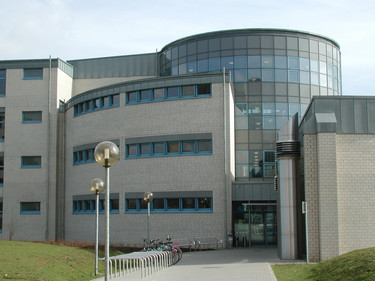
\includegraphics{content/images/52_Foto_FHDortmund_Gebaeude.jpg}
	\caption{Geb�ude des FB4}
	\label{fig:FB4Bild}
\end{figure}


%************** FORMELN ******************
\subsection{Formeln}
Einfache Formeln oder einzelne mathematische Symbole k�nnen durch das Dollar-Zeichen \$ eingebunden werden: \$ Formel \$. Eine so erstellte Formel k�nnte folgenderma�en aussehen:
\begin{center}
	$X(z) = \sum_{n=-\infty}^\infty ( x[n]  * r^{-n} ) * e^{-j\omega n}$ \\
\end{center}

Werden in dem Dokument viele Formeln verwendet und soll bei Bedarf noch einmal darauf zur�ckgegriffen werden k�nnen, macht es Sinn Formeln zu nummerieren. Dazu m�ssen Formeln folgenderma�en eingebunden werden:\\

\textbackslash begin\{equation\textbraceright \\
	\noindent\hspace*{10mm} Hier die Formel\\
\textbackslash end\{equation\textbraceright

Das Ergebnis k�nnte so aussehen:
\begin{equation}
		t-t_{0}=\sqrt{\frac{l}{g}}\int_{0}^{\varphi}{\frac{d\psi}{\sqrt{1-k^{2}\sin^{2} {\psi}}}} = \sqrt{\frac{l}{g}} F(k,\varphi)
\end{equation}
		\section{Zeichnungen}

Die folgenden Zeichnungen wurden mit den \LaTeX -Zusatzpaketen pgf und tikz erstellt. Sie stellen sehr m�chtige Werkzeuge zur Verf�gung um Diagramme und Grafiken aller Art zu erstellen. Die Ergebnisse sind professionell und k�nnen, falls n�tig, mit wenig Aufwand ge�ndert werden. Es erfordert nat�rlich eine gewisse Einarbeitung, aber diese wird durch die Resultate schnell wieder aufgewogen.
Eine umfangreiche Anleitung mit vielen weiteren Beispielen findet sich auf \\ \href{http://www.ctan.org/tex-archive/graphics/pgf/base/doc/generic/pgf/pgfmanual.pdf}{http://www.ctan.org/tex-archive/graphics/pgf/base/doc/generic/pgf/pgfmanual.pdf} \\

Es folgen einige Beispiele.


%********************** Zustandsdiagramm *******************
\subsection{Zustandsdiagramm}

Das Zustandsdiagramm (englisch: state diagram) der UML ist eine der dreizehn Diagrammarten dieser Modellierungssprache f�r Software und andere Systeme. Es stellt einen endlichen Automaten in einer UML-Sonderform grafisch dar und wird benutzt, um entweder das Verhalten eines Systems oder die zul�ssige Nutzung der Schnittstelle eines Systems zu spezifizieren.

\begin{figure}[H]
\begin{center}
	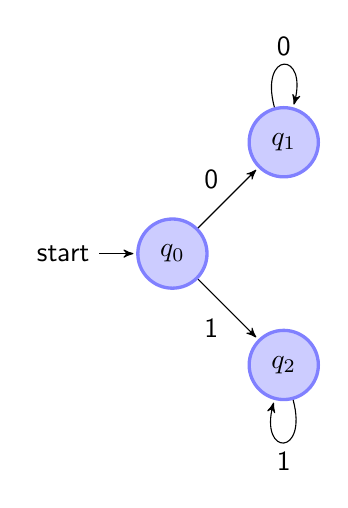
\begin{tikzpicture}[shorten >=1pt,node distance=2cm,on grid,>=stealth', every state/.style={draw=blue!50,very thick,fill=blue!20}]
		\node[state,initial] (q_0) {$q_0$};
		\node[state] (q_1) [above right=of q_0] {$q_1$};
		\node[state] (q_2) [below right=of q_0] {$q_2$};
		\path[->] (q_0) edge node [above left] {0} (q_1)
			edge node [below left] {1} (q_2)
			(q_1) edge [loop above] node {0} ()
			(q_2) edge [loop below] node {1} ();
	\end{tikzpicture}
	\caption{Zustandsdiagramm}
	\label{fig:zustandsdiagramm}
\end{center}
\end{figure}


%********************** Petrinetz *******************
\subsection{Petrinetz}
Ein Petri-Netz ist ein mathematisches Modell von nebenl�ufigen Systemen. Es ist eine formale Methode der Modellierung von Systemen bzw. Transformationsprozessen. Die urspr�ngliche Form der Petri-Netze nennt man auch Bedingungs- oder Ereignisnetz. Petri-Netze wurden durch Carl Adam Petri in den 1960er Jahren definiert. Sie verallgemeinern wegen der F�higkeit, nebenl�ufige Ereignisse  darzustellen, die Automatentheorie.

\begin{figure}[H]
\begin{center}
		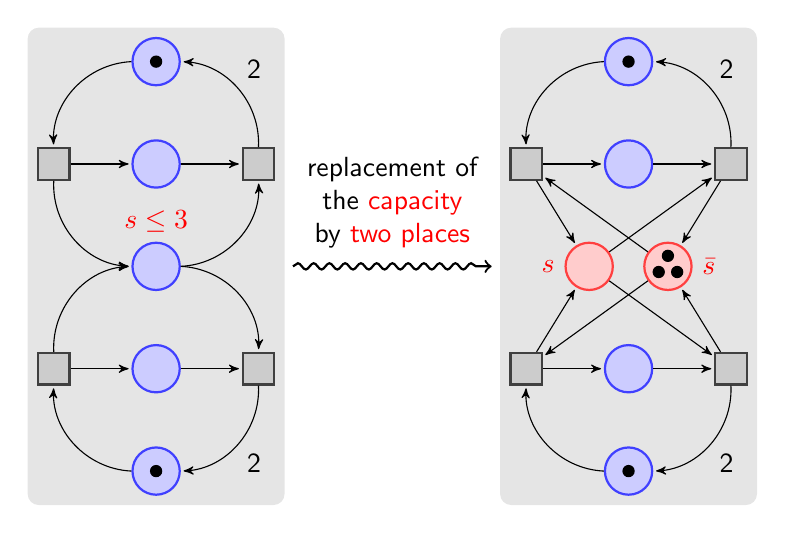
\begin{tikzpicture}
			[node distance=1.3cm,on grid,>=stealth',bend angle=45,auto,
			every place/.style= {minimum size=6mm,thick,draw=blue!75,fill=blue!20},
			every transition/.style={thick,draw=black!75,fill=black!20},
			red place/.style= {place,draw=red!75,fill=red!20},
			every label/.style= {red}]
			\node [place,tokens=1] (w1) {};
			\node [place] (c1) [below=of w1] {};
			\node [place] (s) [below=of c1,label=above:$s\le 3$] {};
			\node [place] (c2) [below=of s] {};
			\node [place,tokens=1] (w2) [below=of c2] {};
			\node [transition] (e1) [left=of c1] {}
			edge [pre,bend left] (w1)
			edge [post,bend right] (s)
			edge [post] (c1);
			\node [transition] (e2) [left=of c2] {}
			edge [pre,bend right] (w2)
			edge [post,bend left] (s)
			edge [post] (c2);
			\node [transition] (l1) [right=of c1] {}
			edge [pre] (c1)
			edge [pre,bend left] (s)
			edge [post,bend right] node[swap] {2} (w1);
			\node [transition] (l2) [right=of c2] {}
			edge [pre] (c2)
			edge [pre,bend right] (s)
			edge [post,bend left] node {2} (w2);
			\begin{scope}[xshift=6cm]
			\node [place,tokens=1] (w1') {};
			\node [place] (c1') [below=of w1'] {};
			\node [red place] (s1') [below=of c1',xshift=-5mm]
			[label=left:$s$] {};
			\node [red place,tokens=3] (s2') [below=of c1',xshift=5mm]
			[label=right:$\bar s$] {};
			\node [place] (c2') [below=of s1',xshift=5mm] {};
			\node [place,tokens=1] (w2') [below=of c2'] {};
			\node [transition] (e1') [left=of c1'] {}
			edge [pre,bend left] (w1')
			edge [post] (s1')
			edge [pre] (s2')
			edge [post] (c1');
			\node [transition] (e2') [left=of c2'] {}
			edge [pre,bend right] (w2')
			edge [post] (s1')
			edge [pre] (s2')
			edge [post] (c2');
			\node [transition] (l1') [right=of c1'] {}
			edge [pre] (c1')
			edge [pre] (s1')
			edge [post] (s2')
			edge [post,bend right] node[swap] {2} (w1');
			\node [transition] (l2') [right=of c2'] {}
			edge [pre] (c2')
			edge [pre] (s1')
			edge [post] (s2')
			edge [post,bend left] node {2} (w2');
			\end{scope}
			\begin{pgfonlayer}{background}
			\node (r1) [fill=black!10,rounded corners,fit=(w1)(w2)(e1)(e2)(l1)(l2)] {};
			\node (r2) [fill=black!10,rounded corners,fit=(w1')(w2')(e1')(e2')(l1')(l2')] {};
			\end{pgfonlayer}
			\draw [shorten >=1mm,-to,thick,decorate,
			decoration={snake,amplitude=.4mm,segment length=2mm,
			pre=moveto,pre length=1mm,post length=2mm}]
			(r1) -- (r2) node [above=1mm,midway,text width=3cm,text centered]
			{replacement of the \textcolor{red}{capacity} by \textcolor{red}{two places}};
		\end{tikzpicture}
	\caption{Petrinetz}
	\label{fig:petrinetz}
	\end{center}
\end{figure}



%********************** Graph *******************
\subsection{Graph}

Ein Graph besteht in der Graphentheorie anschaulich aus einer Menge von Punkten, zwischen denen Linien verlaufen. Die Punkte nennt man Knoten  oder Ecken, die Linien nennt man meist Kanten, manchmal auch B�gen. Auf die Form der Knoten und Kanten kommt es im allgemeinen dabei nicht an. Knoten und Kanten k�nnen auch mit Namen versehen sein, dann spricht man von einem benannten Graphen.

\begin{figure}[H]
	\begin{center}
	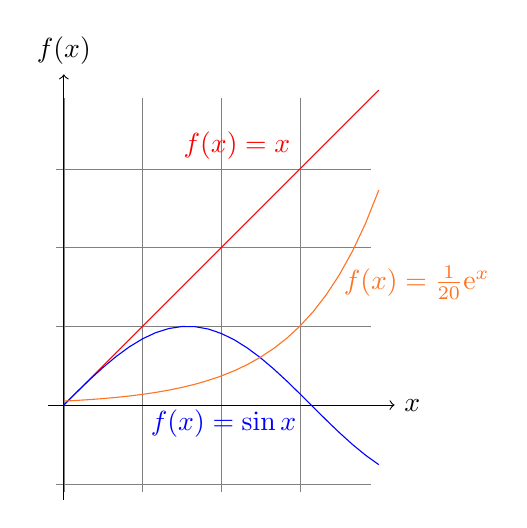
\begin{tikzpicture}[domain=0:4,label/.style={postaction={
	decorate,
	decoration={
		markings,
		mark=at position .75 with \node #1;}}}]
	\draw[very thin,color=gray] (-0.1,-1.1) grid (3.9,3.9);
	\draw[->] (-0.2,0) -- (4.2,0) node[right] {$x$};
	\draw[->] (0,-1.2) -- (0,4.2) node[above] {$f(x)$};
	\draw[red,label={[above left]{$f(x)=x$}}] plot (\x,\x);
	\draw[blue,label={[below left]{$f(x)=\sin x$}}] plot (\x,{sin(\x r)});
	\draw[orange,label={[right]{$f(x)= \frac{1}{20} \mathrm e^x$}}] plot (\x,{0.05*exp(\x)});
\end{tikzpicture}
	\caption{Graph}
	\label{fig:graph}
	\end{center}
\end{figure}

		%Tabellen%
\section{Tabellen}

Hier finden sich einige Beispiele f�r Tabellen und etwas Blindtext drumrum, damit sie nicht so verloren aussehen :)

Lorem ipsum dolor sit amet, consectetuer adipiscing elit. Aenean commodo ligula eget dolor. Aenean massa. Cum sociis natoque penatibus et magnis dis parturient montes, nascetur ridiculus mus. Donec quam felis, ultricies nec, pellentesque eu, pretium quis, sem. Nulla consequat massa quis enim. Donec pede justo, fringilla vel, aliquet nec, vulputate eget, arcu. In enim justo, rhoncus ut, imperdiet a, venenatis vitae, justo. Nullam dictum felis eu pede mollis pretium. Integer tincidunt. Cras dapibus. Vivamus elementum semper nisi. Aenean vulputate eleifend tellus. Aenean leo ligula, porttitor eu, consequat vitae, eleifend ac, enim. 

\begin{table}[ht]
\begin{tabular}{|l|l|l|}
\hline
Author & Title & Year \\
\hline
\hline
Philip K. Dick & Minority Report & 1956 \\
\hline
Philip K. Dick & Do Androids Dream of Electric Sheep? & 1968 \\
\hline
Philip K. Dick & A Scanner Darkly & 1977 \\
\hline
Neal Stephenson & Snow Crash & 1992 \\
\hline
Neal Stephenson & The Diamond Age & 1995 \\
\hline
Neal Stephenson & Cryptonomicon & 1999 \\
\hline
\end{tabular}
\caption{Einfache Tabelle}
\end{table}

Auch gibt es niemanden, der den Schmerz an sich liebt, sucht oder w�nscht, nur, weil er Schmerz ist, es sei denn, es kommt zu zuf�lligen Umst�nden, in denen M�hen und Schmerz ihm gro�e Freude bereiten k�nnen. Um ein triviales Beispiel zu nehmen, wer von uns unterzieht sich je anstrengender k�rperlicher Bet�tigung, au�er um Vorteile daraus zu ziehen? Aber wer hat irgend ein Recht, einen Menschen zu tadeln, der die Entscheidung trifft, eine Freude zu genie�en, die keine unangenehmen Folgen hat, oder einen, der Schmerz vermeidet, welcher keine daraus resultierende Freude nach sich zieht? Auch gibt es niemanden, der den Schmerz an sich liebt, sucht oder w�nscht, nur, weil er Schmerz ist, es sei denn, es kommt zu zuf�lligen Umst�nden, in denen M�hen und Schmerz ihm gro�e Freude bereiten k�nnen. Um ein triviales Beispiel zu nehmen, wer von uns unterzieht sich je anstrengender k�rperlicher Bet�tigung, au�er um Vorteile daraus zu ziehen? Aber wer hat irgend ein Recht, einen Menschen zu tadeln, der die Entscheidung trifft, eine Freude zu genie�en, die keine unangenehmen Folgen hat, oder einen, der Schmerz vermeidet, welcher keine daraus resultierende Freude nach sich zieht? Auch gibt es niemanden, der den Schmerz an sich liebt, sucht oder w�nscht, nur,

\begin{table}[ht]
\begin{tabular}{|l|l|l|}
\hline
Author & Title & Year \\
\hline
\hline
\multirow{3}{*}{Philip K. Dick} & Minority Report & 1956 \\
\cline{2-3}
 & Do Androids Dream of Electric Sheep? & 1968 \\
\cline{2-3}
 & A Scanner Darkly & 1977 \\
\hline
\multirow{3}{*}{Neal Stephenson} & Snow Crash & 1992 \\
\cline{2-3}
 & The Diamond Age & 1995 \\
\cline{2-3}
 & Cryptonomicon & 1999 \\
\hline
\end{tabular}
\caption{Einfache Tabelle mit zusammengefassten Zeilen}
\end{table}

Zwei flinke Boxer jagen die quirlige Eva und ihren Mops durch Sylt. Franz jagt im komplett verwahrlosten Taxi quer durch Bayern. Zw�lf Boxk�mpfer jagen Viktor quer �ber den gro�en Sylter Deich. Vogel Quax zwickt Johnys Pferd Bim. Sylvia wagt quick den Jux bei Pforzheim. Polyfon zwitschernd a�en M�xchens V�gel R�ben, Joghurt und Quark. "Fix, Schwyz! " qu�kt J�rgen bl�d vom Pa�. Victor jagt zw�lf Boxk�mpfer quer �ber den gro�en Sylter Deich. Falsches �ben von Xylophonmusik qu�lt jeden gr��eren Zwerg. Heiz�lr�cksto�abd�mpfung.

\begin{table}[h] 
\begin{tabular}{l c c rrrrrrr}    % creating 10 columns 
\hline\hline                         % inserting double-line  
Audio &Audibility & Decision &
\multicolumn{7}{c}{Sum of Extracted Bits} \\ 
[0.5ex]    
\hline                  % inserts single-line  % Entering 1st row  
& &soft &1 & $-1$ & 1 & 1 & $-1$ & $-1$ & 1  \\
[-1ex] 
\raisebox{1.5ex}{Police} & \raisebox{1.5ex}{5}&hard &  2 & $-4$ & 4 & 4 & $-2$ & $-4$ & 4 \\[1ex]  % Entering 2ndrow 
& &soft & 1 & $-1$ & 1 & 1 & $-1$ & $-1$ & 1  \\
[-1ex] \raisebox{1.5ex}{Beethoven} & \raisebox{1.5ex}{5}& hard &8 & $-8$ & 2 & 8 & $-8$ & $-8$ & 6 \\[1ex]  % Entering 3rd row 
& &soft & 1 & $-1$ & 1 & 1 & $-1$ & $-1$ & 1  
\\[-1ex] \raisebox{1.5ex}{Metallica} & \raisebox{1.5ex}{5}& hard &4 & $-8$ & 8 & 4 & $-8$ & $-8$ & 8 \\[1ex]  % [1ex] adds vertical space \hline                         % inserts single-line 
\end{tabular} 
\label{tab:PPer} 
\caption{Noch eine sehr h�bsche Tabelle}  % title name of the table 
\end{table} 

Zwei flinke Boxer jagen die quirlige Eva und ihren Mops durch Sylt. Franz jagt im komplett verwahrlosten Taxi quer durch Bayern. Zw�lf Boxk�mpfer jagen Viktor quer �ber den gro�en Sylter Deich. Vogel Quax zwickt Johnys Pferd Bim. Sylvia wagt quick den Jux bei Pforzheim. Polyfon zwitschernd a�en M�xchens V�gel R�ben, Joghurt und Quark. "Fix, Schwyz! " qu�kt J�rgen bl�d vom Pa�. Victor jagt zw�lf Boxk�mpfer quer �ber den gro�en Sylter Deich. Falsches �ben von Xylophonmusik qu�lt jeden gr��eren Zwerg. Heiz�lr�cksto�abd�mpfung. Zwei flinke Boxer jagen die quirlige Eva und ihren Mops durch Sylt. Franz jagt im komplett verwahrlosten Taxi quer durch Bayern. Zw�lf Boxk�mpfer jagen Viktor quer �ber den gro�en Sylter Deich. Vogel Quax zwickt Johnys Pferd Bim. Sylvia wagt quick den Jux
	\chapter{Fazit}
\label{fazit}
In diesem Kapitel wird eine Retrospektive des durchgeführten Projekts gegeben. Dabei wird zwischen dem Ergebnis bei der Erstellung der Applikationen und dem Erreichen der persönlichen Ziele unterschieden.
\section{Ziele / Ergebnisse}
\label{sec:ziele-ergebnisse}
Rückblickend kann das Projekt als ein Erfolg gesehen werden. \\
Aus dem Projekt ist eine umfassende Client-Server-Landschaft entstanden, welche die gesetzten Anforderungen an eine verlässliche mobile Applikation, sowohl in den Aspekten der Benutzerfreundlichkeit als auch der Verlässlichkeit, erfüllt. Sowohl der Server als auch beide Clients haben in den jeweils erstellten Meilensteine alle muss Kriterien erfüllt. Teilweise konnten sogar noch optionale Kann-Kriterien umgesetzt werden. So ist es beispielsweise möglich, sich an der Web \ac{API} zu registrieren oder in der nativen \gls{App} eine Trainingsstatistik aufzubauen. 
Dies ist besonders deshalb bemerkenswert, da die Projektteilnehmenden einen großteils der genutzten Techniken erst erlernen mussten. 
Alle im Projekt erzeugten Ressourcen können über das öffentliche Git-Repository unter \textit{\href{https://github.com/Fanuer/fIT}{https://github.com/Fanuer/fIT}} abgerufen werden. 

%Anfangs wurde ein Überblick über die Aufgabe gegeben und die Systemarchitektur vorgestellt. Darauf aufbauend wurden die verwendeten Technologien erörtert und die Umsetzungen der beiden Applikationen bis zu einem festgelegten Punkt dokumentiert. Die Implementierung des Servers wurde zusätzlich betrachtet. Die anschließende Gegenüberstellung der Apps hat ergeben, dass die Weiterentwicklung der Android-App in Hinsicht auf Sicherheit als einzige Lösung gesehen werden kann.\\
%Deshalb wurde für diese Applikation ein zweiter Meilenstein begonnen, um die Anforderungen an den umzusetzenden Prototypen zu implementieren. 
%Rückblickend kann das Projekt als ein großer Erfolg gesehen werden. Die eingangs formulierten Ziele konnten vollständig umgesetzt werden. Zudem wurden teilweise noch Funktionen umgesetzt, die über das formulierte Ziel hinaus gehen.\\
%Zusammenfassend ist es nun mit dem Prototypen möglich den kompletten Funktionsumfang der nativen Android-App auch im \textit{Oflline}-Modus nutzen zu können. 
\section{Erkenntnisse}
\label{sec:erkenntnisse}
Der Erkenntnisgewinn dieser Arbeit ist beträchtlich. \\
Es wurden vorwiegend unbekannte und für die Autoren neue Technologien verwendet. Die Einarbeitung geschah in den meisten Fällen reibungslos. Dies wurde gerade zu Anfang des Projekts jedoch auch als Risiko empfunden, welches ein Problem in der Umsetzung hätte verursachen können. Diese Zweifel waren jedoch im nach hinein unbegründet. \\
Die Tatsache, dass dieses Projekt von zwei Personen durchgeführt wurde, ergab sich als enormer Vorteil. Dies gestattet, punktuell Spezialwissen zu erwerben, was jeweils der anderen Person vermittelt werden musste. Dadurch wurde der Lerneffekt nochmals verstärkt und Zusammenhänge leichter vertieft.\\
Ebenfalls wurde von beiden Projektteilnehmer als sinnvoll erachtet, dass eine Komplettlösung für ein größeres Feld an Aufgaben, nämlich mobile Applikationen, geschaffen werden musste. Das meint, dass nicht nur einer Cache-Komponente für ein bestehendes System erstellt wurde, sondern jede Komponenten für die Realisierung der Systemlandschaft erstellt, verwaltet und veröffentlicht werden musste.\\
Somit konnte sich ein Einblick über alle anfallenden Arbeitsschritte zur Umsetzung einer mobilen Applikation geschaffen werden. 
\section{Ausblick}
\label{sec:ausblick}
Die Grundlage für den Ausbau dieses Projektes zu einer marktreifen \gls{App} ist gegeben. Der dahinter liegende Server ist stark genug, um eine größere Last an Anfragen zu bewältigen. Zum Ausbau dieses Projekts muss die \gls{Android}-\gls{App} weiterentwickelt werden. \\
Die Umsetzung aller wichtiger Funktionen wurde jeweils an mindestens einem Beispiel im Messeprototyp dargestellt und muss demnach nur noch auf die fehlenden Funktionalitäten übertragen werden.\\
Durch den nun tieferen Einblick in die Technologien sollte sich dieser Aufwand in Grenzen halten.\\
Auf Seiten dies Servers müssen hauptsächlich Sicherheitsfunktionen weiterentwickelt werden, um die Web API öffentlich nutzbar zumachen. Zu diesen Funktionen zählen beispielsweise die Validierung von ClientIDs, die Einschränkung eingehender Anfragen durch \ac{CORS} und die Signierung von Tokens. \\
Darüber hinaus kann eine Weiterentwicklung der \ac{App} dazu führen, dass die Web \ac{API} Ressourcen erweitert werden muss. 
	
	% ----------------- Ende des eigentlichen Textes
	

	%Verzeichnisse erstellen
  \chapter*{Abkürzungsverzeichnis}
\addcontentsline{toc}{chapter}{Abkürzungsverzeichnis}  
\begin{acronym}[Visual Studio] %Längster Begriff
\setlength{\itemsep}{-\parsep}
	\acro{.apk}{Android Package}
	\acro{ACL}{Access Control Lists}
	\acro{AES}{Advanced Encryption Standard}
	\acro{AJAX}{Asynchronous JavaScript and XML}	
	\acro{ANR}{Application Not Responding}
	\acro{API}{Application Programming Interface}
	\acro{CORS}{Cross-origin resource sharing}
	\acro{CRUD}{Create Read Update Delete}	
	\acro{CSS}{Cascading Style Sheet}
	\acro{DLL}{Dynamic Link Library}
	\acro{DRAM}{Dynamischer \ac{RAM}}
	\acro{HTML}{Hypertext Markup Language}	
	\acro{HTTP}{Hypertext Transfer Protocol}	
	\acro{HTTPS}{Hyper Text Transfer Protocol Secure}	
	\acro{IDE}{Integrated Development Environment}
	\acro{JSON}{JavaScript Object Notation}	
	\acro{JWT}{\ac{JSON} Web Token}	
	\acro{MSSQL}{Microsoft SQL Server}
	\acro{MVC}{Model-View-Controller}	
	\acro{MVVM}{Model-View-ViewModel}
	\acro{OR-Mapper}{objekt-relationaler Mapper}
	\acro{PCL}{Portable Class Library}
	\acro{RAM}{Random Access Memory}
	\acro{RBAC}{Role Based Access Control}	
	\acro{REST}{Representational State Transfer}	
	\acro{SPA}{Single Page Application}
	\acro{SRAM}{Statischer \ac{RAM}}
	\acro{TCP}{Transmission Control Protocol}
	\acro{URI}{Uniform Resource Identifier}		
	\acro{URL}{Uniform Resource Locator}		
	\acro{Visual Studio}{Microsoft Visual Studio 2015 Community Edition}		
	\acro{VM}{Virtuelle Maschine}
	\acro{Web-App}{mobil-optimierte Webseite}
	\acro{XML}{Extensible Markup Language}
\end{acronym}

	\listoffigures
	\listoftables
	\lstlistoflistings
	
	\appendix
	\nocite{*} 
	
	%Literaturverzeichnis erstellen
	\bibliography{bib/bib}

	%\chapter{Anhang}
\label{cha:anhang}

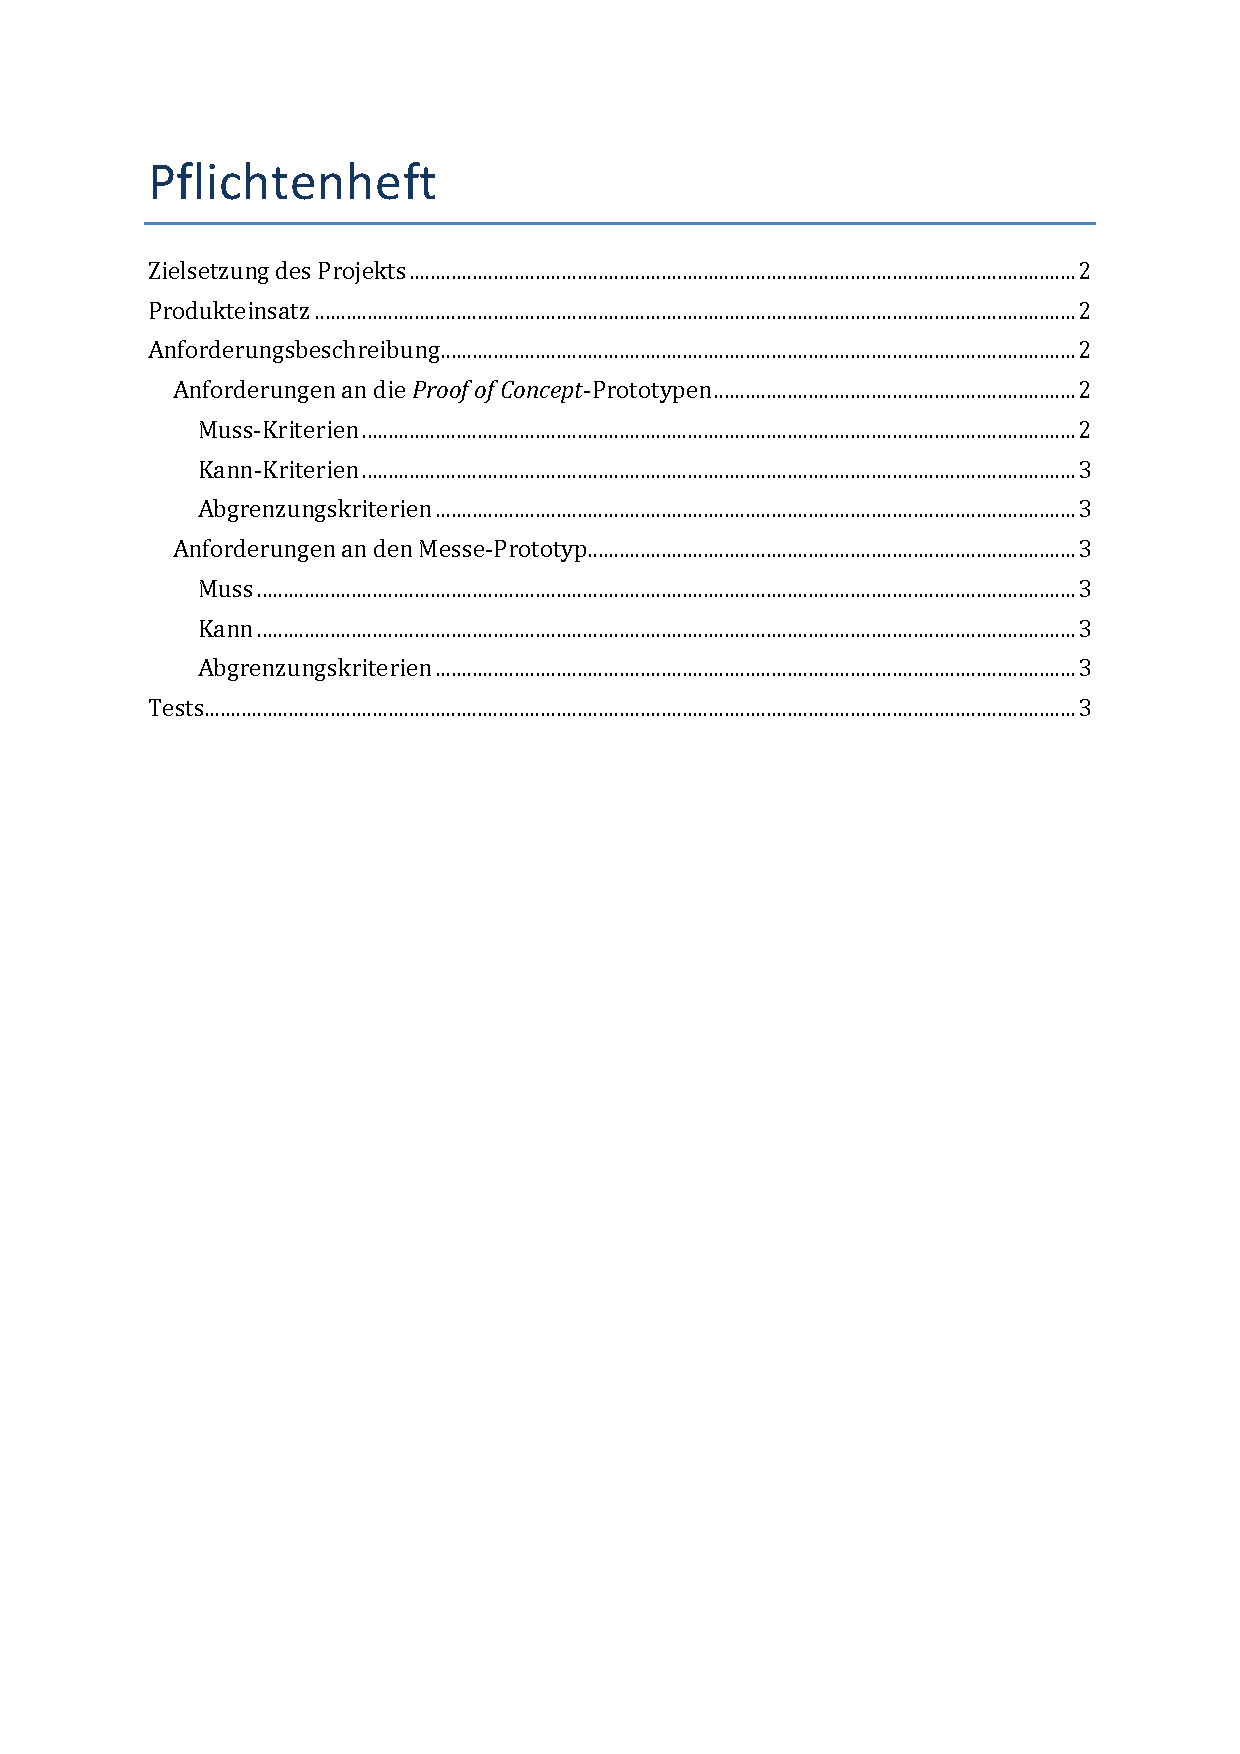
\includepdf[pages={-},frame= true, scale=0.68, pagecommand=\section{Pflichtenheft}\label{sec:Pflichtenheft}]{content/additional/Pflichtenheft.pdf}

\section{Cache Post}
\label{sec:cachePost}

%CachePush-Bild
\begin{figure}[!h]
\centering
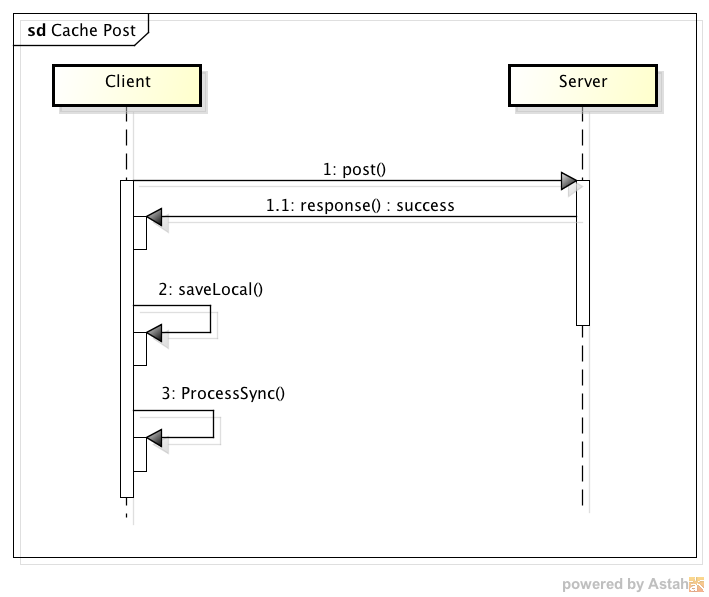
\includegraphics[width=0.8\linewidth]{content/images/Cache-Post}
\caption{Hochladen zum Server}
\label{pic:cachePost}
\end{figure}

\section{User-Story in der nativen App}
\label{sec:UserStory}
%Startseite
\begin{figure}[!h]
\centering
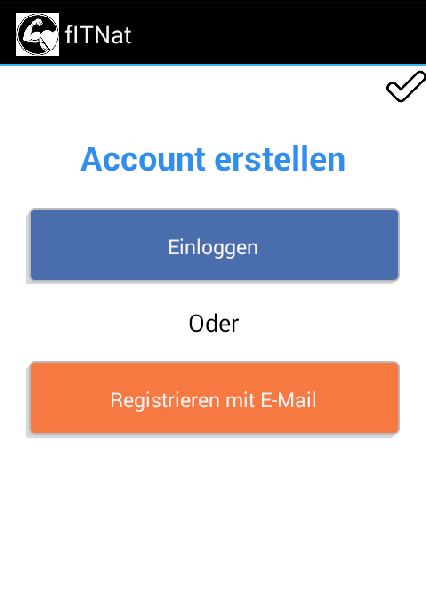
\includegraphics[width=0.5\linewidth]{content/images/App/Startseite}
\caption{Startseite}
\label{pic:natAppStartseite}
\end{figure}
%Login
\begin{figure}[!h]
\centering
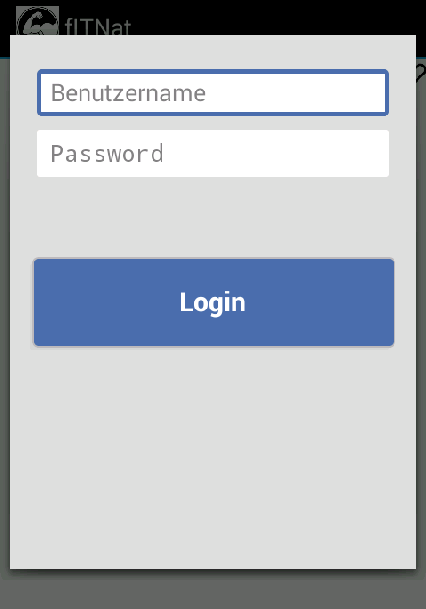
\includegraphics[width=0.5\linewidth]{content/images/App/SignIn}
\caption{Login}
\label{pic:natAppLogin}
\end{figure}
%Reistrierung
\begin{figure}[!h]
\centering
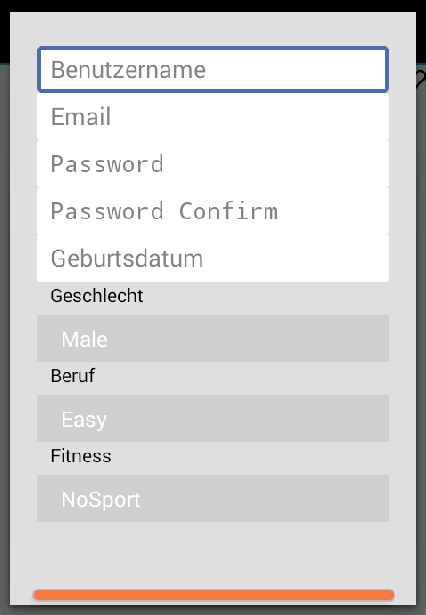
\includegraphics[width=0.5\linewidth]{content/images/App/SignUp}
\caption{Registrierung}
\label{pic:natAppRegistrierung}
\end{figure}
%Trainingspläne
\begin{figure}[!h]
\centering
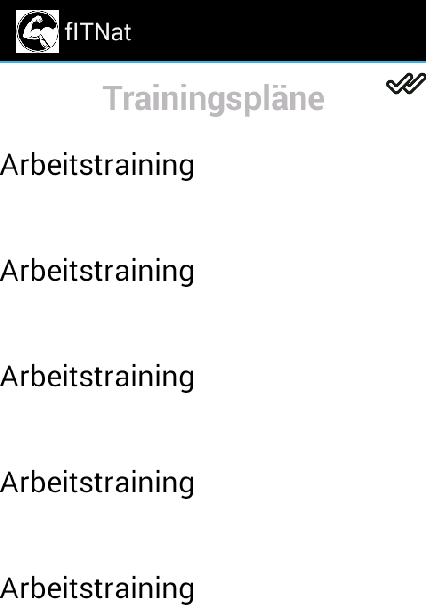
\includegraphics[width=0.5\linewidth]{content/images/App/Trainingsplan}
\caption{Übersicht der Trainingspläne}
\label{pic:natAppTrainingspläne}
\end{figure}
%Übungen
\begin{figure}[!h]
\centering
\includegraphics[width=0.5\linewidth]{content/images/App/Übungen}
\caption{Übersicht der Übungen}
\label{pic:natAppÜbungen}
\end{figure}
%Training
\begin{figure}[!h]
\centering
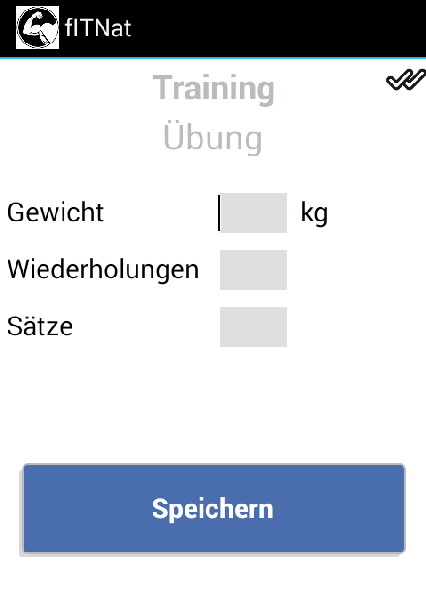
\includegraphics[width=0.5\linewidth]{content/images/App/Training}
\caption{Training}
\label{pic:natAppTraining}
\end{figure}
%Statistik
\begin{figure}[!h]
\centering
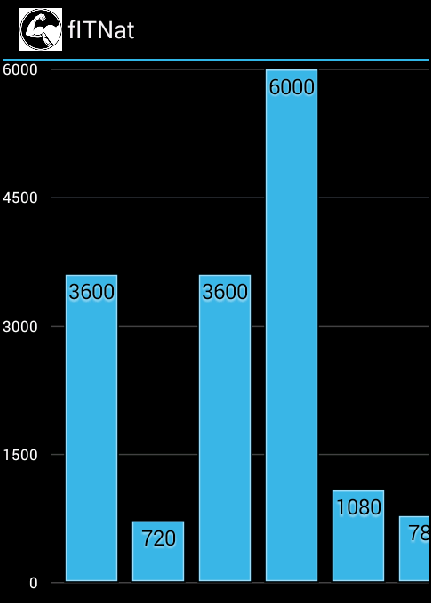
\includegraphics[width=0.5\linewidth]{content/images/App/Statistik}
\caption{Statistik}
\label{pic:natAppStatistik}
\end{figure}

\section{Funktionsumfang}
\label{natAppFunktionen}
	\chapter{Eidesstattliche Erkl�rung}
Gem�� �\,17,(5) der BPO erkl�re ich an Eides statt, dass ich die vorliegende Arbeit
selbst�ndig angefertigt habe. Ich habe mich keiner fremden Hilfe bedient und keine
anderen, als die angegebenen Quellen und Hilfsmittel benutzt. Alle Stellen, die
w�rtlich oder sinngem�� ver�ffentlichten oder nicht ver�ffentlichten Schriften und
anderen Quellen entnommen sind, habe ich als solche kenntlich gemacht. Diese
Arbeit hat in gleicher oder �hnlicher Form noch keiner Pr�fungsbeh�rde vorgelegen.
\vspace{3\baselineskip}\\
Dortmund, \thedate \hfill \theauthor

\vspace{1cm}
\section*{Erkl�rung}
Mir ist bekannt, dass nach �\,156~StGB bzw. �\,163~StGB eine falsche Versicherung
an Eides Statt bzw. eine fahrl�ssige falsche Versicherung an Eides Statt mit
Freiheitsstrafe bis zu drei Jahren bzw. bis zu einem Jahr oder mit Geldstrafe
bestraft werden kann.
\vspace{3\baselineskip}\\
Dortmund, \thedate \hfill \theauthor

\end{document}
